\chapter{Results and analysis}

\section{PSNR SCORE}
The Peak-signal-to-noise ratio (PSNR) score is an engineering term for the ratio between the maximum possible power of a signal and the power of corrupting noise that affects the fidelity of its representation.PSNR score is used for Image super-resolution works as an accuracy measurment even though they can't model human perceptual similarity

PSNR score is easily defined via the mean squared error(MSE).Given the high resolution image $I^{HR}$ and super resolved image $I^{SR}$,MSE is defined as:
\begin{equation}
MSE = \frac{1}{mn}\sum_{i=0}^{m-1}\sum_{j=0}^{n-1}{[I^{SR} - I^{HR}]}^2
\end{equation}
The PSNR (in dB) is defined as:
\begin{equation}
PSNR = 20 log_{10}(MAX_I) - 10 log_{10}(MSE)
\end{equation}
Here, $MAX_i$ is the maximum possible pixel value of the image.In our case $MAX_I = 255$ 

The accuracy of the network where tested against two bechmarks 'Set5' and 'Set14' and the corresponding average psnr score for each of them where calculated
\begin{center}
\begin{tabular}{|m{3cm} | m{3cm} | m{3cm} | m{3cm} |}
 \hline
 \textbf{Dataset} & \textbf{SRRESNET} & \textbf{SRGAN} \textbf{Bicubic}\\
 \hline
 Set5 &33.096&32.84 \\
\hline
 Set14 &31.95 &31.90 \\
 \hline
\end{tabular}
\end{center}
\section{Result Visualization}
The Images from standard benchmark where downsampled using bicubic interpolation and where upscaled using both trained SRResNet Model(consisting only the generator) and SRGAN Model.Some samples of the results are shown in figure: \ref{fig:sampleoutput} 
\begin{figure}[h]
\centering
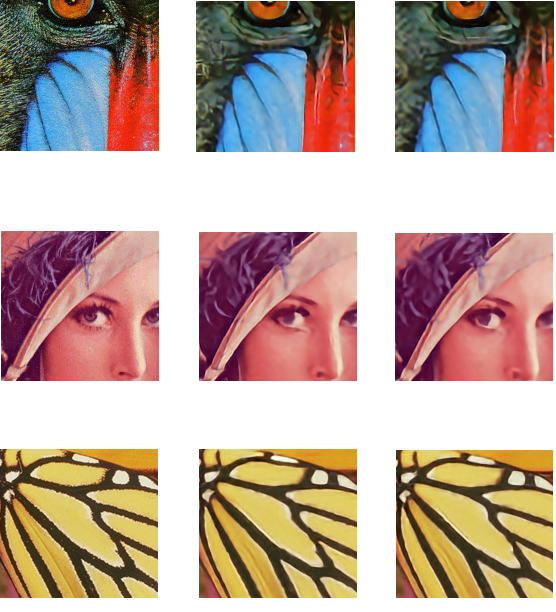
\includegraphics[scale=0.5]{sample_output}
\caption{Comparision of sample Ground Truth Image, SRGAN Image and SRRESNET Image}
\label{fig:sampleoutput}
\end{figure}

\begin{figure}[h]
\centering
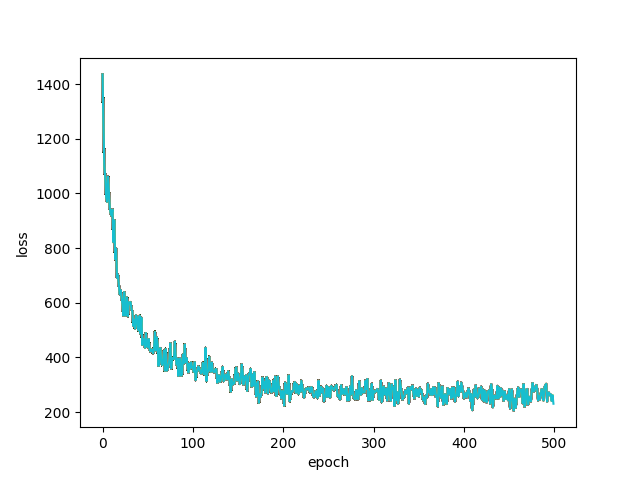
\includegraphics[scale=0.8]{srresnet_loss}
\caption{Plot of loss against number of Epochs for SRResNet}
\label{fig:srresnetloss}
\end{figure}

\begin{figure}[h]
\centering
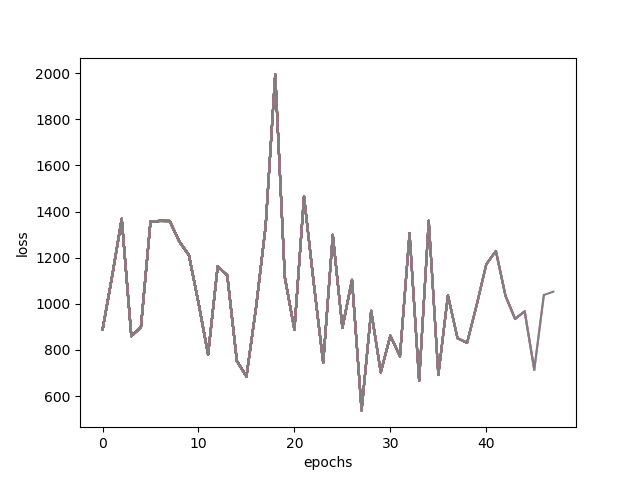
\includegraphics[scale=0.8]{srgan_loss}
\caption{Plot of loss against number of Epochs for SRGAN}
\label{fig:srganloss}
\end{figure}